%&program=pdflatex
%&encoding=UTF-8 Unicode
\documentclass[a4paper]{llncs}
\usepackage{llncsdoc}

%% Deutsche Anpassungen %%%%%%%%%%%%%%%%%%%%%%%%%%%%%%%%%%%%%
\usepackage[ngerman]{babel}
\usepackage[T1]{fontenc}
\usepackage[utf8]{inputenc}
%\usepackage{fontspec}
%\setromanfont[Mapping=tex-text,Alternate=1,Ligatures={Common,Diphthong}]{Palatino} 

% Mateh
\usepackage{amsmath}
\usepackage{amssymb}

% Paket für Graphiken
\usepackage[pdftex]{graphicx}

%\Paket für Hyperlinks
\usepackage[
bookmarks=true,
bookmarksopen=true,
bookmarksnumbered=true,
breaklinks=true,
colorlinks=true,
linkcolor=black,
anchorcolor=black,
citecolor=black,
filecolor=black,
menucolor=black,
pagecolor=black,
urlcolor=black
]{hyperref}

\begin{document}

\title{Clustering of DBPedia Subjects}
\subtitle{Seminar Map/Reduce Algorithms on Hadoop}
\author{Robert Pfeiffer, Tobias Schmidt}
\institute{Fachgebiet Informationssysteme\\Hasso-Plattner-Institut für Softwaresystemtechnik\\Prof.-Dr.-Helmert-Str. 2-3\\14482 Potsdam, Deutschland\\31. August 2009}

\maketitle

\section{Einleitung}
Mit der fortschreitenden Nutzung der Computertechnik in allen Lebensbereichen steigt auch das zu bearbeitende Datenvolumen stetig an. Damit auf immer größeren Datenmengen weiterhin effizient Berechnungen ausgeführt werden können, wurde von Google\footnote{\url{http://www.google.com/}} ein Berechnungsmodell namens MapReduce entwickelt. Mit dieser Architektur ist es möglich, Berechnungen auf mehrere Computer zu verteilen und parallel ablaufen zu lassen.

Im Seminar \emph{Map/Reduce Algorithms on Hadoop}\footnote{\url{http://www.hpi.uni-potsdam.de/naumann/lehre/ss_09/mapreduce_algorithms_on_hadoop.html}} haben wir uns mit dem in Java implementieten, MapReduce-Framework \emph{Hadoop}\footnote{\url{http://hadoop.apache.org/}} auseinandergesetzt und einen Algorithmus implementiert, der eine Menge von Objekten anhand ihrer Ähnlichkeit gruppiert.

\section{Grundlagen}

\subsubsection{MapReduce}
MapReduce ist ein Programmiermodell, welches erstmals 2004 vorgestellt wurde \cite{DG04} und Prinzipien funktionaler Programmierung aufgreift. 
Der MapReduce Ansatz besteht im Allgemeinen aus zwei Funktionen: \emph{Map} und \emph{Reduce}. In der Map-Funktion wird ein Problem in mehrere Teilprobleme zerlegt, die idealerweise parallel und unabhängig voneinander ausgeführt werden.
Anschließend werden die Ergebnisse der Teilprobleme in der Reduce-Funktion wieder zu einem Gesamtergebnis zusammengesetzt.

Die Map-Funktion erwartet als Eingabe Schlüssel-Wert-Paare und gibt neue Schlüssel-Wert-Paare als Ergebnis aus.
Die Reduce-Funktion erhält als Eingabe einen Schlüssel und alle dazugehörigen Werte.
Diese Werte werden je nach vorgegebener Berechnung zusammengeführt und dem Schlüssel zugeordnet.
Reduce gibt anschließend wiederum Schlüssel-Wert-Paare zurück.

\subsubsection{Hadoop}
Hadoop ist ein in Java implementiertes Open Source Framework, welches auf dem MapReduce-Modell basiert.
Die Kernkomponenten stellen Schnittstellen für verteilte Dateioperationen und Ein-/Ausgabe sowie ein verteiltes Dateisystem (HDFS) bereit.
Eine Aufgabe, die auf der Hadoop-Plattform ausgeführt werden soll, ist ein Job.
Dieser besteht aus einer Map- sowie einer Reduce-Funktion.
Ein Job-Tracker überwacht den Gesamtfortschritt eines MapReduce-Jobs,
generiert die Map- und Reduce-Tasks und verteilt diese an die einzelnen Nodes im Hadoop-Cluster.
% Das Hadoop Framework übernimmt die Zerlegung der Eingabedatei und ruft für jedes Schlüssel-Wert-Paar die angegebene Map-Funktion auf.
% Der Task-Tracker überwacht den Fortschritt auf den Nodes und teilt ihnen bei Bedarf weitere Tasks zu. 

\subsubsection{DBPedia}
Das \emph{DBPedia}-Projekt\footnote{\url{http://dbpedia.org/}} extrahiert Informationen aus der Online-Enzyklopädie \emph{Wikipedia}\footnote{\url{http://www.wikipedia.org/}}, bereitet diese auf und stellt diese strukturiert zur freien Verfügung.
Als Hauptquelle für Informationen in der \emph{DBPedia} sind die Infoboxen zu nennen, die in vielen \emph{Wikipedia}-Artikeln auf der rechten Seite existieren.

Die Daten werden als RDF-Tripel der Form $(Subject, Attribut, Wert)$ in der DBPedia gehalten (z.B. $(Berlin, populationTotal, 3429300)$).
Es gibt ca. 44.000 verschiedene Attribute in der DBPedia, wobei davon auszugehen ist, dass gleiche Attribute auch die gleiche Semantik haben. Dadurch lassen sich aus dem Gruppieren der Subjekte nach ähnlichen Attributmengen möglicherweise semantische Rückschlüsse in Bezug auf die Subjekt-Gruppen ziehen.

\subsubsection{Clustering}
Algorithmen, beziehungsweise Verfahren, die eine Menge von Objekten zu Gruppen (Cluster) mit jeweils ähnlichen Eigenschaften zusammenfassen, bezeichnet man als Clusteranalyseverfahren. % Heuristik?
% Es gibt eine ganze Reihe von unterschiedlichen Ansätzen zur Analyse, die alle unterschiedliche Vor- und Nachteile haben.
% Grundsätzlich unterscheidet man zwischen partitionierenden und hierarchischen Analyseverfahren.

Für viele Clusterverfahren wird ein Abstandsmaß benötigt. Dieses gibt für zwei Objekte einen Wert zurück, der angibt, wie weit die beiden Objekte voneinander entfernt sind. Kleinere Werte beschreiben üblicherweise geringere Abstände. 
%Es gibt verschiedene Abstandsmaße, die für unterschiedlichen Daten unterschiedlich gute Ergebnisse liefern.
Als Beispiele sind das \emph{Euklidische Abstandsmaß} und die \emph{Jaccard-Distanz} zu nennen.

\subsubsection{k-Means}
Wir haben das partitionierende Clusteranalyseverfahren \emph{k-Means} angewendet.
\emph{k-Means} zeichnet sich durch seine hohe Geschwindigkeit aus, liefert jedoch nicht zwingend die optimale Lösung. Desweiteren muss man bei \emph{k-Means} die Anzahl der gewünschten Cluster im Vorfeld vorgeben.

Zu Beginn des Algorithmus wählt man zufällig die gewünschte Anzahl von Clustern aus der Objektmenge aus. Diese Objekte bilden die initialen Clusterzentren. Die zufällige Auswahl der Clusterzentren bewirkt, dass bei verschiedenen Programmdurchläufen mit gleichen Eingabedateien unterschiedliche Cluster berechnet werden können. Nach der Wahl der Clusterzentren beginnt der iterative Teil des Algorithmus.

Für jedes Objekt wird mit Hilfe eines Abstandsmaßes der Abstand zu jedem Clusterzentrum berechnet. Anschließend wird das Objekt demjenigen Cluster zugeordnet, zu dessen Clusterzentrum es den geringsten Abstand aufweist.
Nachdem alle Objekte einem Cluster zugeordnet worden sind, wird das neue Clusterzentrum bestimmt, indem der Schwerpunkt aller dem Cluster zugeordneten Objekte berechnet wird.

Dieser Vorgang wird solange wiederholt, bis nach einer Iteration kein Objekt mehr einem anderen Clusterzentrum zugeordnet wird.
%Alternativ kann auch eine prozentuale Schranke festgelegt werden (zum Beispiel: wiederhole bis weniger als 2\% der Objekte einem anderen Cluster zugeordnet werden). %Das kommt unten doch 

\subsubsection{Jaccard-Distanz}
Die Jaccard-Distanz ist ein Abstandsmaß, dass die Ähnlichkeit zwischen Mengen angibt. Dabei sind zwei Mengen einander ähnlicher, je mehr Elemente sie gemeinsam haben. Die Jaccard-Distanz von einer Menge zu sich selbst ist Null.

%Die Jaccard-Distanz basiert auf dem Jaccard-Index, dem Quotienten aus Schnitt- und Vereinigungsmenge zweier Mengen.

$$J_{\delta}(A,B) = %1 - J(A,B) = 
{ { |A \cup B| - |A \cap B| } \over |A \cup B| }$$

Ein Vorteil der Jaccard-Distanz gegenüber dem euklidischen Abstandsmaß ist, dass Elemente, die in den jeweiligen Mengen enthalten sind, stärker berücksichtigt werden, als nicht enthaltene Elemente. Beim Euklidischen Abstand beeinflussen Elemente, die in beiden Mengen fehlen oder vorhanden sind, das Abstandsmaß gleich.

\subsubsection{Fuzzy-Mengen}
\label{sec:Fuzzy}
Da die Clusterzentren gemittelte Werte enthalten, können sie nicht wie die Subjekte als einfache Mengen dargestellt werden.
Stattdessen werden Fuzzy-Mengen benutzt, in denen ein Element zu einem gewissen Grad zwischen 0 und 1 enthalten sein kann.
Dies wird durch die Funktion $\mu : M \times E \rightarrow [0,1] $ beschrieben. Dabei bedeutet $m(A,e) = 0$ soviel wie $ e \not\in A $ und $m(A,e) = 1$ entspricht $ e \in A $ aus der normalen Mengenlehre.

Die Identitäten für Schnitt- Vereinigungsmengen in der Mengenlehre \begin{align*}e \in (A \cap B) = (e \in A) \wedge (e \in B)
	\\ e \in (A \cup B) = (e \in A) \vee (e \in B) \end{align*} lauten für Fuzzy-Mengen  \begin{align*}\mu(e, A \cap B) = min(\mu(e, A), \mu(e, B))\\ \mu(e, A \cup B) = max(\mu(e, A), \mu(e, B))  \end{align*}.

Damit lässt sich der Jaccard-Index numerisch auf folgende Weise berechnen:

$P$ sei die Menge aller möglichen Attribute.
$$J_{\delta}(A,B) = \frac{\sum\limits_{p \in P}max\bigl(\mu(p, A)\mu(p, B)\bigr) - min\bigl(\mu(p, A),\mu(p, B))\bigr)}{\sum\limits_{p \in P}max\bigl(\mu(p, A),\mu(p, B))\bigr)}$$

\section{Implementierung}

\subsubsection{Datenformat}
%- Problem: Daten sind große Matrizen\\
%- Vorteile:\\
%    - Hadoop Format, dadurch gibt es bereits ein Interface und Hadoop kann den Input splitten\\
%    - komprimiert\\
%- Nachteile:\\
%    - kodiertes Format, daher für Menschen nicht lesbar\\
%   - keine Information über die Gesamtgröße
Die uns zur Verfügung gestellte Datenmenge ist eine Teilmenge von Ressourcen aus der \emph{DBPedia}.
Da die Werte der RDF-Tripel für das Clustern keine Relevanz besitzen, wurden diese entfernt.
Die Eingabedatei enthält die Subjekte in einem Binärformat. Dabei wird jedes Subjekt durch ein Array von Bits repräsentiert, wobei die Stelle im Array immer ein Attribut repräsentiert. Wenn an einer Stelle ein 1-Bit steht, dann besitzt die Ressource das Attribut, andernfalls nicht.

Da Hadoop die Eingabe in kleinere Teile aufspalten können muss, standen wir vor der Wahl entweder einen entsprechenden Binärparser zu schreiben, oder die Eingabe in ein anderes Format zu überführen.
Da ersteres eine recht aufwändige Aufgabe ist, entschieden wir uns dazu, das \emph{Sequence File} Format zu benutzen, welches speziell für Hadoop entwickelt wurde, und aus Schlüssel-Wert-Paaren von serialisierten Objekten besteht.
\emph{Sequence Files} können von Hadoop aufgesplittet werden und sind komprimierbar. 
Die Originaldatei mit einer Größe von mehr als 120GB konnte somit auf unter 100MB komprimiert werden.
Dies ist vor allem bei der Übertragung der Eingabe auf die einzelnen Nodes im Hadoop-Cluster von großem Vorteil.

\subsubsection{Generierung der Clusterzentren}
Das erste Problem bei der Implementierung des \emph{k-Means} Algorithmus stellte die Generierung der initialen Clusterzentren dar. Hadoop erlaubt es, in einem Programm mehrere Jobs hintereinander auszuführen. Dadurch bestand eine Möglichkeit darin, mittels eines Jobs die Zentren zu generieren und mit Hilfe eines zweiten Jobtyps den iterativen Teil des Algorithmus auszuführen. Die zweite von uns erarbeitete Idee war, die Clusterzentren vor dem Starten des Hadoop-Programmes separat zu generieren und als weiteren Eingabeparameter mitzuliefern. Wir haben uns für dieses Verfahren entschieden, da es zum einen zu diesem Zeitpunkt für uns leichter zu implementieren war und zum anderen durch die einmalige Generierung einen Geschwindigkeitsvorteil darstellt. Für eine finale Version des Programms wäre es jedoch von Vorteil, wenn der Benutzer nicht selbst die Clusterzentren generieren müsste.

% hat auch Vorteile beim evaluieren

\subsubsection{Distributed Cache}
%- Problem: Verteilung der Centroids\\
%- Lösung mittels Distributed Cache\\
%- Vorteile: in Hadoop, synchrone Datenhaltung, wenig Overhead für die restlichen berechnungen\\
%- Nachteile: bricht das Map/Reduce Konzept\\
%- andere Möglichkeit: kartesisches Produkt

Um die Cluster in einer Iteration des \emph{k-Means}-Algorithmus neu zu bestimmen, muss der Abstand jedes Subjektes von jedem Zentrum berechnet werden. Dafür müssen alle Clusterzentren auf jedem Node zur Verfügung stehen.

Anstatt das kartesische Produkt von Clusterzentren und Subjekten zu bilden und anschließend zu verteilen, bestand die Idee darin, den Mappern zu Beginn jeder Iterationvon die Zentren als Parameter zu übergeben. Da die Anzahl der Cluster, und demzufolge auch die der Clusterzentren, viel kleiner als die Anzahl der Subjekte ist, bewirkt dieses Vorgehen einen sehr viel geringeren Kommunikationsaufwand.
% Da im Map-Schritt alle Zentren bekannt sind, kann das nächste Zentrum, und damit die Clusterzugehörigkeit jedes Subjektes, bereits im Map-Schritt bestimmt werden.
% Parameter können jedoch nicht direkt an die Mapper übergeben werden, da die Job-Konfiguarion nicht die Mapper kennt, sondern nur deren Klassennamen. 
% Die Mapper werden erst auf den Knoten erzeugt. Um den Mappern zusätzliche Parameter zu übergeben, werden deshalb zusätzliche Einträge in der Konfiguration sowie der \emph{Distributed Cache} verwendet. 
Der \emph{Distributed Cache} bietet die Möglichkeit, größere Datenmengen an die Knoten zu übermitteln, bevor der eigentliche MapReduce-Zyklus beginnt. Dazu werden die Dateien, die zum \emph{Distributed Cache} hinzugefügt wurden, vom HDFS in das lokale Dateisystem auf den Knoten kopiert. Im Gegensatz zum HDFS stellt der \emph{Distributed Cache} sicher, dass jeder Knoten alle Dateien vollständig erhält, bevor ein MapReduce-Zyklus beginnt.

% Die Knoten können jederzeit auf die lokalen Dateien lesend zugreifen. In unserer Implementierung werden mit der Erzeugung der Mapper die Clusterzentren auf den Knoten ausgelesen und anschließend im Hauptspeicher gehalten.

\subsubsection{Berechnung der Clusterzentren}
\label{sec:BerechnungDerCluster}
% Nachdem die Clusterzentren mittels des \emph{Distributed Cache} auf die einzelnen Knoten verteilt wurden, beginnt die eigentliche Berechnung des .
Der iterative Teil des \emph{k-Means}-Algorithmus lässt sich relativ leicht auf das MapReduce-Schema abbilden.

% Map
Für jedes Subjekt wird eine Map-Funktion aufgerufen.
Diese berechnet den Abstand des Subjektes zu jedem Clusterzentrum, welche mittels \emph{Distributed Cache} zur Verfügung stehen.
Für die Abstandsberechnung haben wir ein Interface \emph{Distance} eingeführt, welches unter anderem die Funktion \emph{between} bereitstellt.
Diese Funktion erwartet als Eingabe zwei Vektoren gleicher Länge und gibt eine reelle Zahl zurück, welche den Abstand zwischen den beiden Vektoren repräsentiert.
Wir haben mit dem \emph{Euklidischen Abstandsmaß} und der \emph{Jaccard-Distanz} zwei verschiedene Implementationen des Interfaces erstellt.
Da für die Berechnung der Jaccard-Distanz beide Vektoren bzw. Mengen Werte aus dem gleichen Wertebereich enthalten müssen,
die Clusterzentren jedoch im Gegensatz zu den Subjekte auch gemittelte Werte enthalten können, haben wir für die Berechnung die in \ref{sec:Fuzzy} beschriebenen Fuzzy-Mengen benutzt.
% Dem Anwender ist es selbst überlassen, welche Implementation er verwenden möchte. Er kann dies durch die Konfigurationsdatei einstellen.
Das Resultat der Map-Funktion ist ein Schlüssel-Wert-Paar, bestehend aus dem Schlüssel des nächsten Clusterzentrums und dem Vektor des Subjektes.

% Reduce
Die Reduce-Phase beginnt, sobald für jedes Subjekt das nächste Clusterzentrum berechnet wurde.
Für jeden eindeutigen Schlüssel wird die Reduce-Funktion genau einmal gerufen.
Als Wert wird eine Liste aller Vektoren übergeben, die diesem Clusterzentrum (sprich diesem Schlüssel) zugeordnet wurden. 
Um den neuen Schwerpunkt des Clusterzentrums zu berechnen,
wird erst die Summe aller Vektoren gebildet und diese anschließend durch die Anzahl der Vektoren dividiert.
Die Reduce-Funktion gibt anschließend ein Schlüssel-Wert-Paar mit dem Schlüssel des Clusters und dem neuen Schwerpunkt als Vektor zurück.

\subsubsection{Abbruch der Iteration}
Da der \emph{k-Means}-Algorithmus erst nach mehreren, im Vorfeld nicht genau bestimmbaren, Iterationen das gewünschte Ergebnis liefert,
muss der in \ref{sec:BerechnungDerCluster} beschriebene Prozess mehrmals ausgeführt werden.
% Allerdings genügt es nicht, nur den Job, der die beschriebenen Map- und Reduce-Funktionen enthält, erneut anzustoßen. Zuvor muss die Ausgabe der Reduce-Funktion, 
% welche die neu berechneten Clusterzentren enthält, in den \emph{Distributed Cache} verschoben werden, 
% um in der nächsten Iteration nicht mit den selben Daten erneut zu rechnen.
Nach der Definition von \emph{k-Means} wird dieser Zyklus beendet, sobald keine bzw. nur noch sehr wenige Subjekte einem anderen Cluster zugeordnet wurden.
Die Umsetzung stellte sich bei unserer Implementation als Problem heraus, da aus Platz- und Geschwindigkeitsgründen keine Informationen über die Zuordnung von Subjekten zu Clustern gespeichert werden. 
% Diese Informationen stehen nur zu Beginn des Reduce-Schrittes zur Verfügung, nicht aber nach Abschluss des Jobs.
Da das Mitführen der Zuordnungen sowie das dauerhafte Speichern sowohl die zwischen den einzelnen Knoten zu übertragenen Datenmengen stark erhöht, als auch in einer komplexeren Programmstruktur gemündet hätte, entschieden wir uns gegen diese Lösung. 
Stattdessen berechnen wir den Fortschritt über die prozentuale Veränderung der Clusterzentren. Bevor die alten Clusterzentren im \emph{Distributed Cache} durch die neuen ersetzt werden, wird für jedes neu berechnete Clusterzentrum der Abstand zum alten Clusterzentrum berechnet.
Die größtmögliche Entfernung von zwei Vektoren entspricht einer Veränderung von 100\%. Sinkt der Durchschnitt aller Veränderungen unter eine vom Benutzer definierte Schranke, so wird der Zyklus abgebrochen.

\section{Evaluierung}

\subsubsection{Laufzeitabschätzung}
Die Laufzeit unserer Implementierung ist abhängig von der Anzahl der Subjekte und der Anzahl der Cluster. Da im Map-Schritt die Abstände aller $k$ Cluster zu allen $s$ Subjekten berechnet werden, liegt die Laufzeitkomplexität des gesamten Map-Teils schrittes in $O(s \cdot k)$. 
Im Reduce-Teil werden alle Cluster gemittelt. Jede Reduce-Funktion berechnet den Mittelwert eines Clusters. 
Je kleiner ein Cluster ist, desto schneller lässt sich sein Schwerpunkt berechnen, doch da jedes Subjekt zu genau einem dieser Cluster gehört, werden alle Subjekte jeweils einmal in eine Berechnung eines Schwerpunktes einbezogen. 
Damit liegt die Komplexität des gesamten Reduce-Schrittes in $O(s)$.
Die Gesamtkomplexität liegt damit in $O(k \cdot s + s)$

Diese theoritische Herleitung der Laufzeitkomplexität wurde in Testreihen mit unterschiedlichen variablen Größen bestätigt.

\subsubsection{Konfiguration}
Bei vorangegangenen Tests wurden starke Unterschiede in der Laufzeit festgestellt, die sich darauf zurückführen lassen, dass die Rechner im Cluster unterschiedlich schnell und unterschiedlich ausgelastet sind. Nach näherer Untersuchung wurde herausgefunden, dass 2 Knoten im Cluster um den Faktor 8 schneller sind, als die übrigen 6 Rechner. Deshalb wurde die Splitsize so konfiguriert, dass die Eingabe auf ca. 22 Map-Tasks verteilt werden konnte. Dadurch wird gewährleistet, dass keiner der 8 Knoten des Clusters auf die anderen lange warten muss.

\subsubsection{Unterschiedliche Subjektanzahl}
Bei dieser Testreihe wurden jeweils Einagbedateien mit 3.500, 7.000, 14.000, 35.000, 70.000, 175.000 und 350.000 Subjekten für den Clustering-Algorithmus verwendet.
Die Anzahl der Cluster betrug dabei konstant 100.
Es wurden jeweils 5 K-Means-Iterationen und ein Output-Job, also insgesamt 6 Hadoop-Jobs ausgeführt. Dadurch fallen Schwankungen bei einzelnen Tasks weniger ins Gewicht.
\begin{figure}[!ht]
\centering
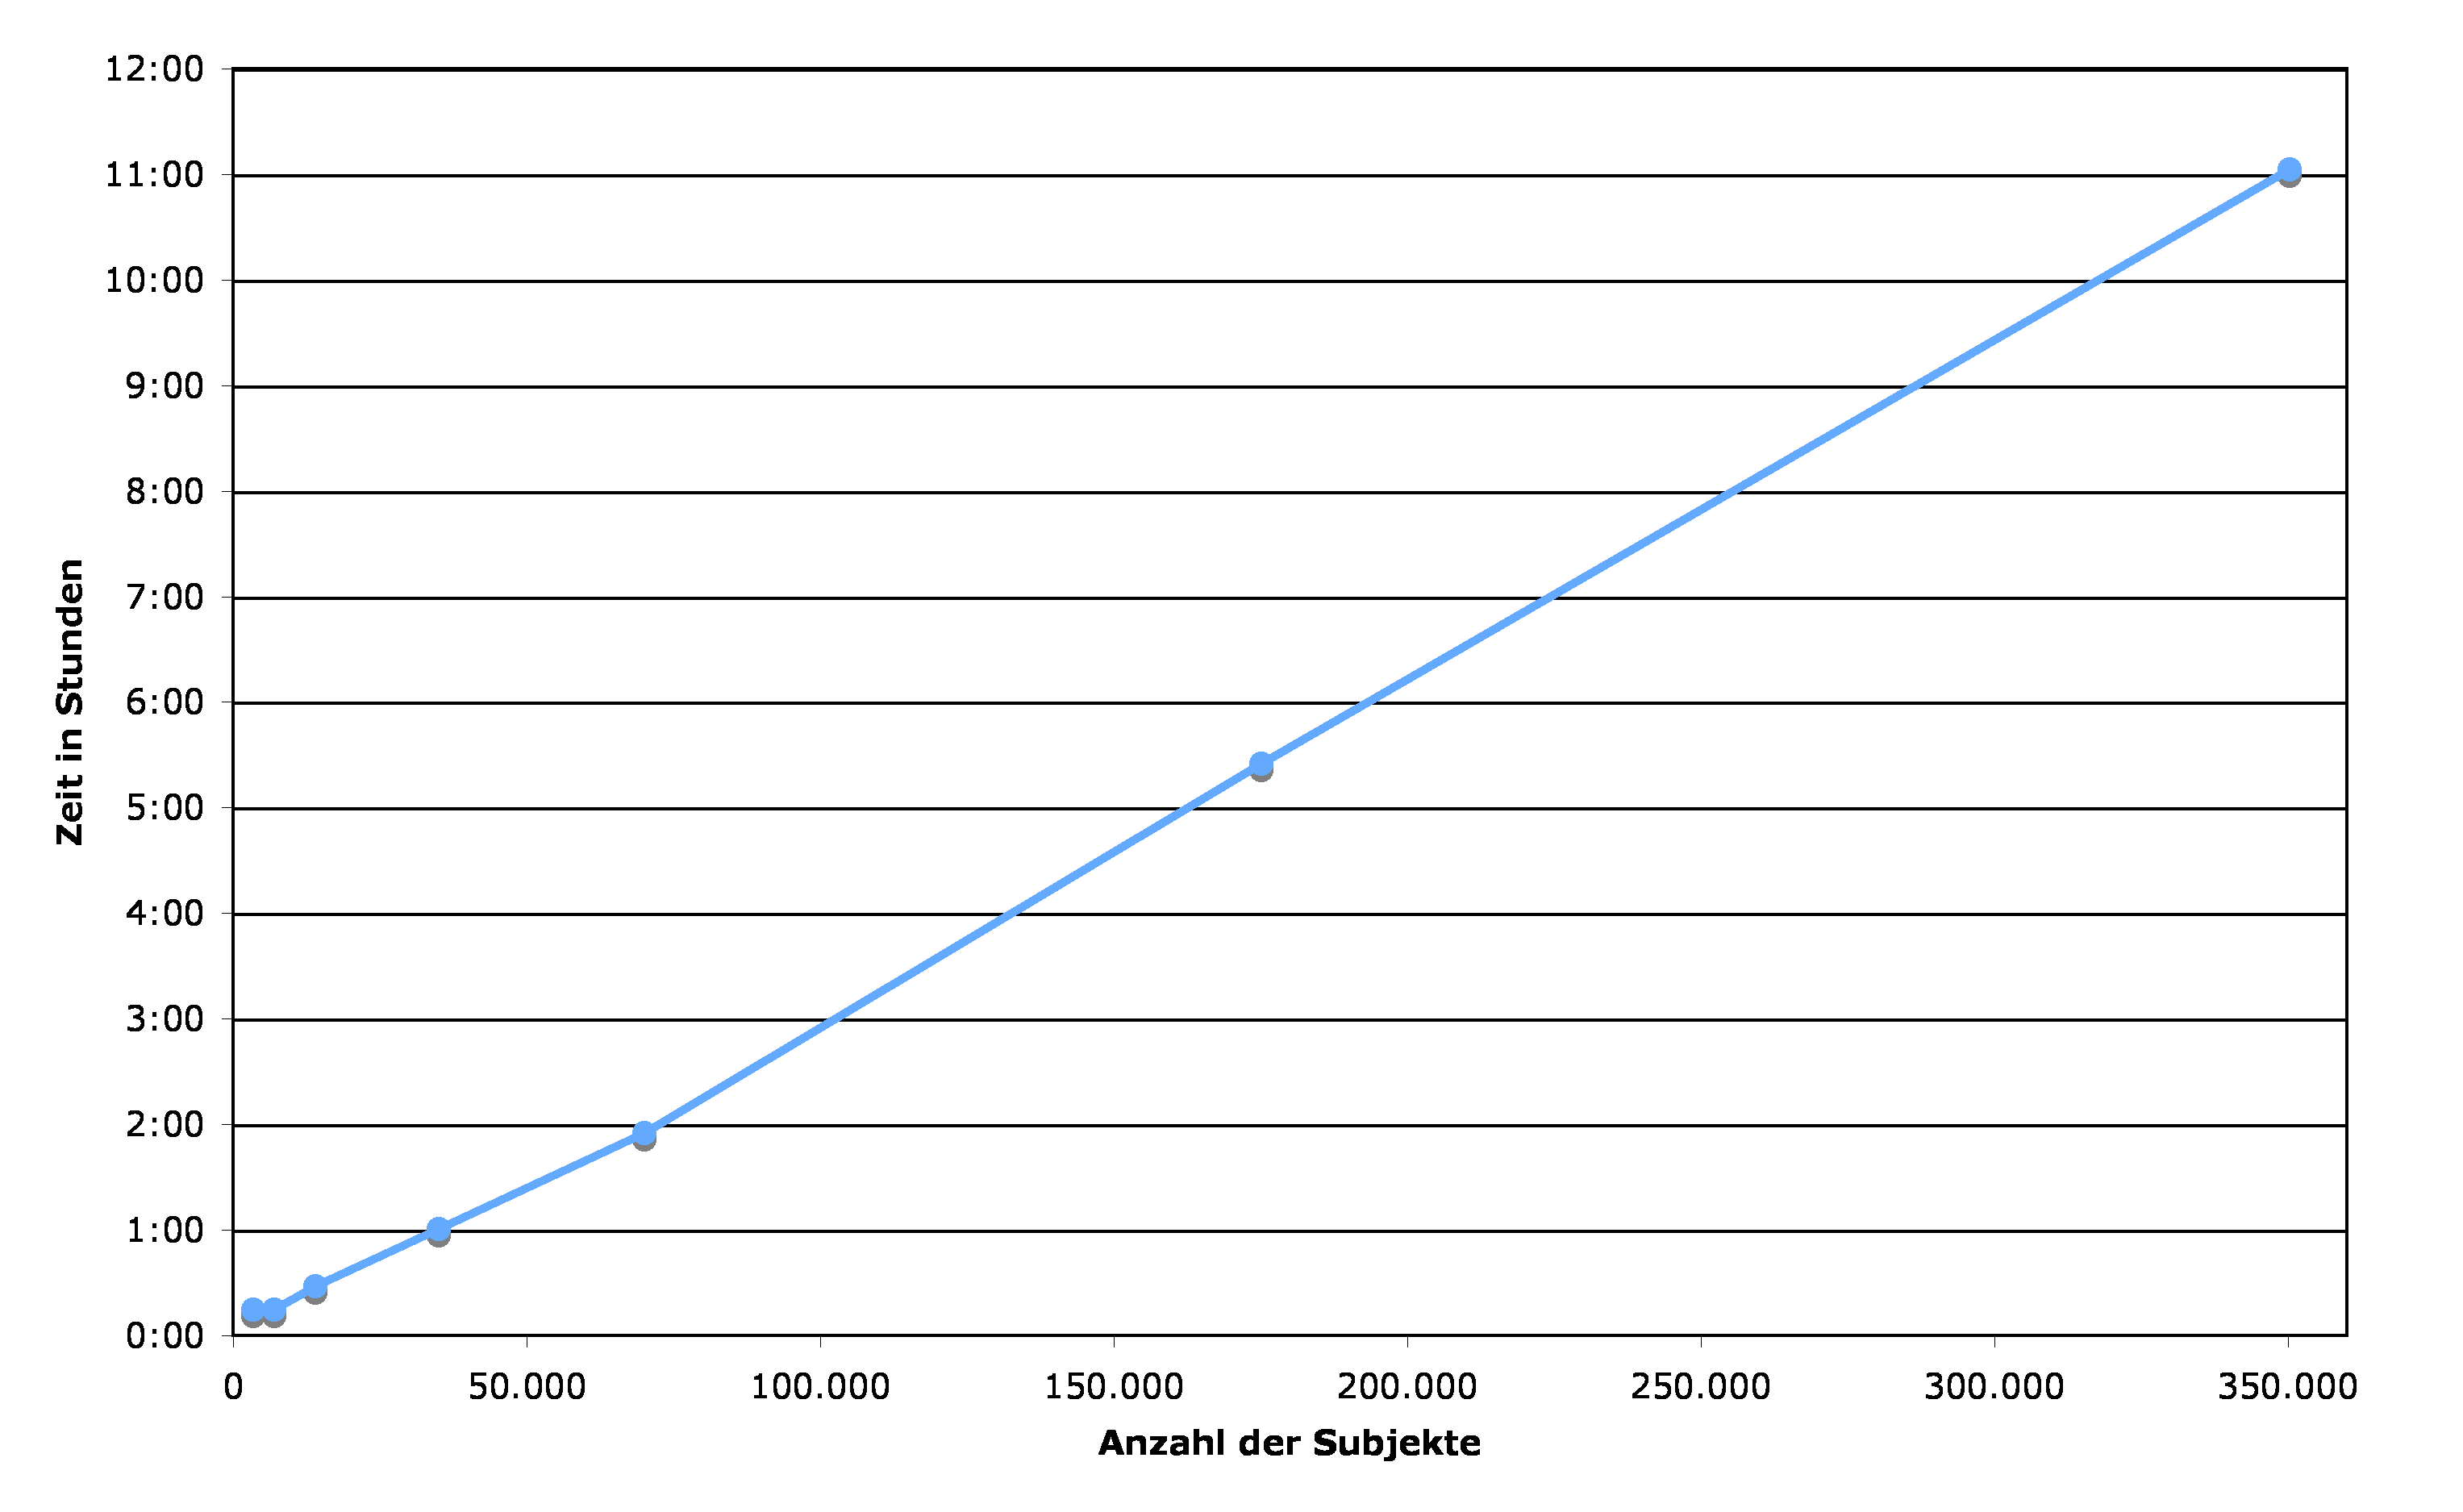
\includegraphics[width=0.99\textwidth]{charts/subjects.png}
\caption{Unterschiedliche Subjektanzahl}
\label{fig:subjects}
\end{figure}
Diese Messreihe in Abbildung \ref{fig:subjects} zeigt, dass die Laufzeit des Algortithmus proportional zur Anzahl der Subjekte ist.

\subsubsection{Unterschiedliche Clusteranzahl}
Bei der zweiten Testreihe lag die Anzahl der Subjekte konstant bei 35.000. Die Anzahl der Cluster wurde zwischen 50, 100, 150, 300, 500 und 1.000 variiert. % nur 50-1000 ?
Dazu wurden jeweils unterschiedliche initiale Clusterzentren generiert.
Es wurden wiederum 5 K-Means-Iterationen und ein Output-Job ausgeführt.
\begin{figure}[!ht]
\centering
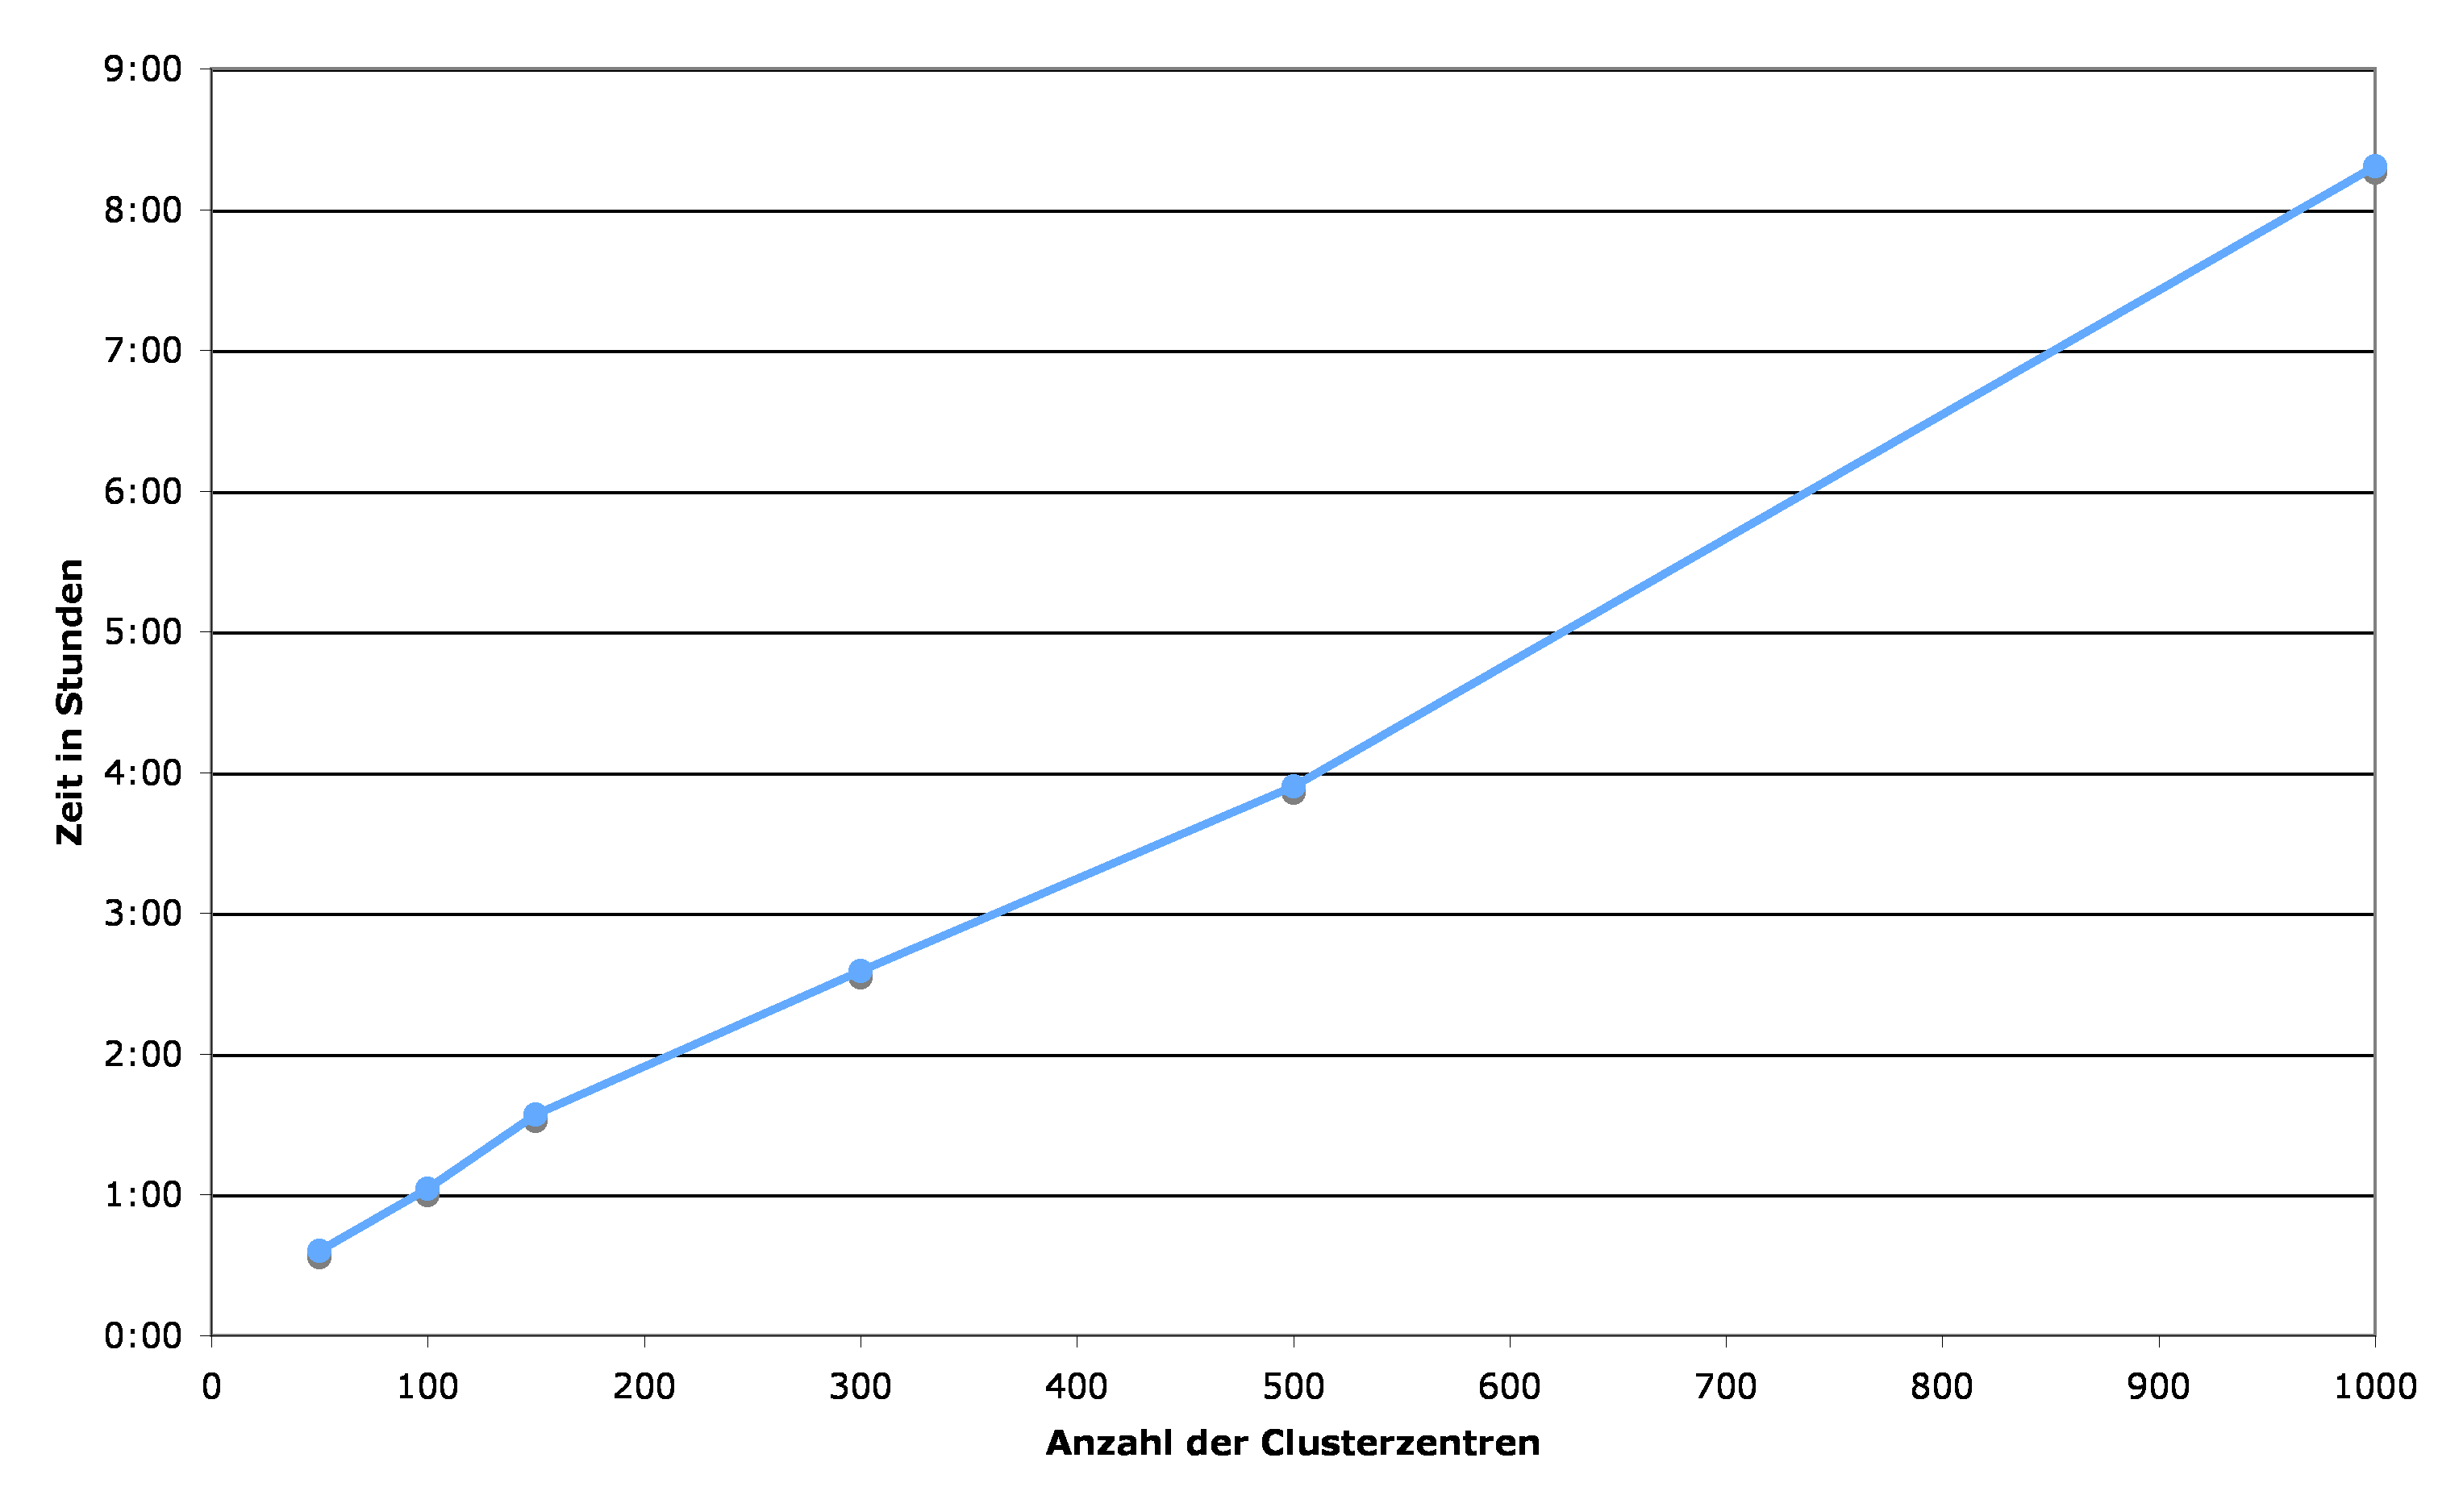
\includegraphics[width=0.99\textwidth]{charts/clustercenters.png}
\caption{Unterschiedliche Anzahl von Clusterzentren}
\label{fig:centers}
\end{figure}
Diese Messreihe in Abbildung \ref{fig:centers} zeigt, dass die Laufzeit des Algortithmus proportional zur Anzahl der Cluster ist.

\subsubsection{Ermittelung der Abbruchbedingung}
%Die Laufzeitabschätzung geht von einer konstanten Anzahl von Iterationen bis zur Konvergenz aus. Um diesen Abstand zu bestimmen, wurde gemessen, wie stark sich die Cluster in jeder Iteration verändern.
Die beiden vorherigen Testreihen wurden mit einer festen Anzahl von Iterationen ausgeführt, um die Laufzeit vergleichen zu können. In dieser Testreihe soll ermittelt werden, wie viele Iterationen nötig sind, bis die durchschnittliche prozentuale Verschiebung der Clusterzentren unter eine definierte Schranke fällt.
Dazu wurden drei Testfälle mit 35.000 Subjekten und 50, 100 bzw. 150 Clustern betrachtet. Bei dem Testfall mit 50 Clustern lag die Abbruchschranke bei 2\% durchschnittlichen Clusterzentrenverschiebungen, bei 100 Clustern bei 1\% und bei 150 Clustern bei 0,5\%.
Durch die logarithmische Skalierung nicht auf den ersten Blick ersichtlich, konvergierten die 3 Testfälle trotz unterschiedlicher Clusteranzahl annähernd gleich schnell.
Wie aus Abbildung \ref{fig:iterations} hervorgeht, nähern sich die Cluster schnell einem relativ stabilen Zustand an.
\begin{figure}[!ht]
\centering
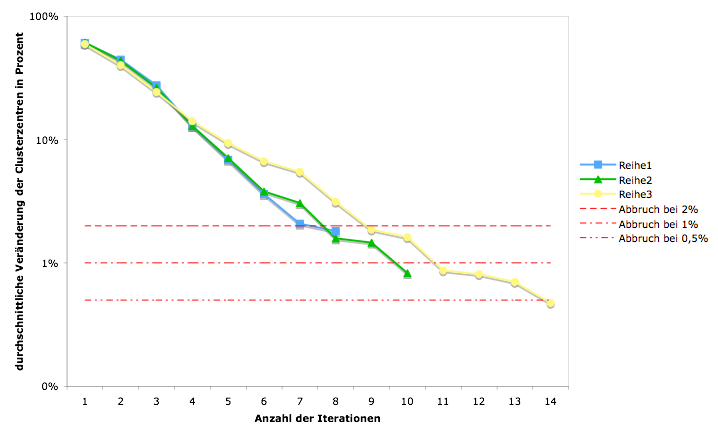
\includegraphics[width=0.99\textwidth]{charts/iterations_log.png}
\caption{Abbruch}
\label{fig:iterations}
\end{figure}

\section{Fazit}
% - Erfahrungen mit verteiltem Rechnen
% - Hadoop kennen gelernt
% - neue Probleme
% - Probleme HDFS vs. lokales Dateisystem

\begin{thebibliography}{------------}

\bibitem[KI2008]{KI2008}
  Segaran, Toby.
  {\em Kollektive Intelligenz}.
  O'Reilly, 2008

\bibitem[DG04]{DG04}
  Dean, Jeffrey; Ghemawat, Sanjay.\\
  {\em MapReduce: Simplified Data Processing on Large Clusters}.\\
  San Francisco, CA, 2004
\bibitem[k-Means]{k-Means}
  \url{http://de.wikipedia.org/wiki/K-Means-Algorithmus}
  
\end{thebibliography}
\end{document}